% ===================================================================
% Slides: Floating Object Solver v2
% Self-consistent body dynamics via monolithic constraint solve
%
% Compile with:  pdflatex slides_v2.tex   (twice for refs)
% Or upload to Overleaf.
% ===================================================================

\documentclass[aspectratio=169, 10pt]{beamer}

\usepackage{amsmath, amssymb, bm}
\usepackage{listings}
\usepackage[table]{xcolor}
\usepackage{tikz}
\usetikzlibrary{matrix, positioning, fit, backgrounds, arrows.meta}
\usepackage{booktabs}
\usepackage{array}
\usepackage{makecell}
\usepackage{colortbl}

%% ---------- Theme & colours ----------
\usetheme{default}
\setbeamertemplate{navigation symbols}{}
\setbeamertemplate{footline}[frame number]

\definecolor{primarycol}{HTML}{1F3A60}
\definecolor{accentcol}{HTML}{E86A4F}
\definecolor{softbg}{HTML}{F2F4F8}
\definecolor{codekw}{HTML}{1F3A60}
\definecolor{codestr}{HTML}{198038}
\definecolor{codecmt}{HTML}{808080}

\setbeamercolor{title}{fg=primarycol}
\setbeamercolor{frametitle}{fg=primarycol}
\setbeamercolor{structure}{fg=primarycol}
\setbeamercolor{alerted text}{fg=accentcol}
\setbeamercolor{block title}{fg=white, bg=primarycol}
\setbeamercolor{block body}{bg=softbg}

\setbeamerfont{frametitle}{size=\Large, series=\bfseries}
\setbeamerfont{title}{size=\LARGE, series=\bfseries}

%% ---------- Code listings ----------
\lstset{
    basicstyle=\ttfamily\scriptsize,
    keywordstyle=\color{codekw}\bfseries,
    commentstyle=\color{codecmt}\itshape,
    stringstyle=\color{codestr},
    language=Python,
    breaklines=true,
    showstringspaces=false,
    columns=fullflexible,
    keepspaces=true,
    frame=none,
    numbers=none,
    escapeinside={(*}{*)},
}

%% ---------- Math shortcuts ----------
\newcommand{\Fr}{\mathrm{Fr}}
\newcommand{\We}{\mathrm{We}}
\newcommand{\Rey}{\mathrm{Re}}
\newcommand{\xx}{\mathbf{x}}
\newcommand{\bb}{\mathbf{b}}
\newcommand{\uu}{\mathbf{u}}
\newcommand{\ww}{\mathbf{w}}
\newcommand{\dd}{\,\mathrm{d}}
\newcommand{\Order}{\mathcal{O}}
\newcommand{\eqn}[1]{\textcolor{accentcol}{\textbf{#1}}}

\title{Floating Object Solver v2}
\subtitle{Self-consistent body dynamics via a monolithic constraint solve}
\author{Wongyung}
\institute{LNS Floating Project}
\date{\today}

\begin{document}

% ===================================================================
\frame{\titlepage}

% ===================================================================
\begin{frame}{Outline}
\begin{enumerate}
    \item Motivation: from prescribed motion to self-consistent dynamics
    \item Physical model: Helmholtz decomposition + body coupling
    \item Monolithic numerical formulation
    \item Python implementation
    \item Concrete examples and validation
    \item Limitations and future work
\end{enumerate}
\vspace{1em}
\small\textit{Goal: every equation traceable to \texttt{floating\_object\_v2.py}.}
\end{frame}

% ===================================================================
% PART 1 — CONTEXT
% ===================================================================

\begin{frame}{Problem setup}
\begin{columns}[T]
\column{0.55\textwidth}
\begin{itemize}
    \item 2D domain, periodic in $x$
    \item Viscous fluid below, free surface above
    \item \textbf{Flat-bottomed rigid body} sits on surface
    \item Body has half-width $a$, mass $m$ (per unit length)
    \item Non-slip at bottom, $z=-D$
    \item At $t=0$: body in contact with surface
\end{itemize}

\column{0.45\textwidth}
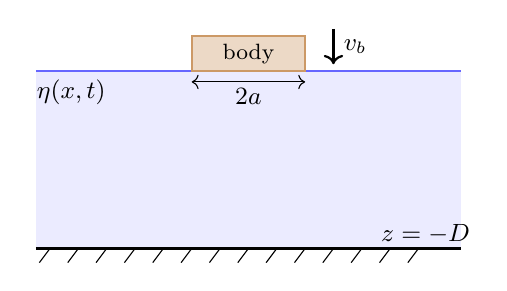
\begin{tikzpicture}[scale=0.9]
    % fluid
    \fill[blue!8] (0,-2.5) rectangle (6,0);
    % surface
    \draw[blue!60, thick] (0,0) -- (6,0);
    % bottom
    \draw[thick] (0,-2.5) -- (6,-2.5);
    \foreach \x in {0.2,0.6,...,5.8}
        \draw (\x,-2.5) -- (\x-0.15,-2.7);
    % body
    \fill[brown!30, draw=brown!80, thick] (2.2, 0) rectangle (3.8, 0.5);
    \node at (3.0, 0.25) {\footnotesize body};
    % arrows
    \draw[->, thick] (4.2, 0.6) -- (4.2, 0.1) node[right, midway]{\small $v_b$};
    \draw[<->] (2.2, -0.15) -- (3.8, -0.15);
    \node at (3.0, -0.35) {\small $2a$};
    % labels
    \node at (0.5, -0.3) {\small $\eta(x,t)$};
    \node at (5.5, -2.3) {\small $z=-D$};
\end{tikzpicture}
\end{columns}

\vspace{0.6em}
\small\textbf{Output we want:} body trajectory $z_b(t)$, body velocity $v_b(t)$, surface elevation $\eta(x,t)$, surface pressure $p_s(x,t)$ — all computed self-consistently.
\end{frame}

% ===================================================================
\begin{frame}{v1 vs v2 at a glance}
\begin{center}
\renewcommand{\arraystretch}{1.25}
\small
\begin{tabular}{@{}p{0.28\textwidth}p{0.33\textwidth}p{0.33\textwidth}@{}}
\toprule
 & \textbf{v1 (\texttt{floating\_object.py})} & \textbf{v2 (\texttt{floating\_object\_v2.py})} \\
\midrule
Body motion & \textbf{Prescribed}: $z_b(t)=-\mathrm{draft}+A\sin(\omega t)$ & \textbf{Computed}: $M\ddot z_b = -M/\Fr + \int p_s\,\dd x$ \\
Role of body & Wavemaker (forced oscillator) & Rigid body with real dynamics \\
Surface pressure $p_s$ & Not computed (ad-hoc) & \textbf{Lagrange multiplier} enforcing no-penetration \\
Free-surface BC under body & Overwrite $\eta \leftarrow z_b(t)$ & Geometric constraint + kinematic match + horizontal no-slip \\
Unknowns per step & $\eta,\phi,w^3,w^1$ & $\eta,\phi,w^3,w^1,\ p_s,\ z_b,\ v_b$ \\
Instability risk & Stable (forced) & Fully implicit $\Rightarrow$ no added-mass issues \\
\bottomrule
\end{tabular}
\end{center}

\vspace{0.5em}
\begin{block}{Key insight}
All new equations are \emph{linear with constant coefficients} $\Rightarrow$ the monolithic prefactorisation trick carries over.
\end{block}
\end{frame}

% ===================================================================
% PART 2 — PHYSICAL MODEL
% ===================================================================

\begin{frame}{Helmholtz decomposition of the velocity field}
\begin{block}{Idea (Galeano-Rios, Milewski, Vanden-Broeck, JFM 2017)}
Split the velocity field into irrotational + vortical parts:
\[
\uu(x,z,t) \;=\; \nabla\phi(x,z,t) \;+\; \ww(x,z,t), \qquad
\nabla \cdot \ww = 0.
\]
\end{block}

\begin{itemize}
    \item $\phi$: velocity potential. Potential flow $\Rightarrow \Delta \phi = 0$ in the bulk.
    \item $\ww = (w^1, w^3)$ in 2D; $w^2 = 0$ by symmetry.
    \item Each component of $\ww$ diffuses: $\partial_t w^i = \nu \Delta w^i$.
    \item Coupling between the two fields happens at boundaries (surface, bottom).
\end{itemize}

\vspace{0.5em}
\small Why: bulk dynamics dominated by potential flow; viscous effects concentrated near boundaries $\Rightarrow$ efficient linear PDE system instead of full nonlinear Navier--Stokes.
\end{frame}

% ===================================================================
\begin{frame}{Bulk equations (dimensionless)}
In the fluid domain $-D \le z \le 0$:
\begin{block}{Potential}
\[
\Delta \phi = 0 \qquad \text{(Laplace's equation — eq.~2.15a)}
\]
\end{block}

\begin{block}{Vortical components}
\[
\partial_t w^i \;=\; \frac{1}{\Rey}\,\Delta w^i, \qquad i = 1, 3  \qquad \text{(heat equations — eq.~2.15b)}
\]
\end{block}

\begin{itemize}
    \item $\Delta$ = full 2D Laplacian $\partial_{xx} + \partial_{zz}$
    \item $\Delta_H = \partial_{xx}$ = horizontal Laplacian (surface operator)
    \item Reynolds number $\Rey = U L_c / \nu$ controls viscous diffusion
\end{itemize}
\end{frame}

% ===================================================================
\begin{frame}{Free-surface boundary conditions (outside body)}
At $z=0$, for $x \notin$ body:
\begin{align}
  \partial_t \eta &= \partial_z \phi + w^3 &&\text{(2.15c: kinematic)} \\[-0.2em]
  \partial_t \phi_s &= -\tfrac{\eta}{\Fr} + \tfrac{1}{\We}\kappa[\eta]
      + \tfrac{2}{\Rey}\Delta_H \phi_s - \tfrac{2}{\Rey} \partial_z w^3 &&\text{(2.15d: dynamic, $p_s=0$)} \\[-0.2em]
  \partial_t w^3 &= \tfrac{2}{\Rey}\Delta_H\!\big(\partial_z \phi + w^3\big) &&\text{(2.15e: vorticity)}\\[-0.2em]
  \partial_z w^1 &= -\big(\partial_{xz}\phi + \partial_x w^3\big) &&\text{(2.11a: stress-free)}
\end{align}

\vspace{0.3em}
\small
$\phi_s(x,t) \equiv \phi(x,0,t)$ is the surface value of the potential; $\kappa[\eta] \approx \partial_{xx}\eta$ is the linearised curvature.
\vspace{0.5em}

\begin{alertblock}{Remark}
In this v2 implementation, \alert{equation (2.15e) is solved directly} — we do \emph{not} use the simplified diagnostic $w^3 = \tfrac{2}{\Rey}\Delta_H \eta$.
\end{alertblock}
\end{frame}

% ===================================================================
\begin{frame}{Under the body: three new constraints}
\footnotesize Let $\mathcal{B}(t) = \{x : |x - x_c| < a\}$ = wetted region.

\begin{block}{(1) Geometric constraint — replaces free-surface kinematic}
\[
\eta(x,t) \;=\; z_b(t) \qquad \forall\, x \in \mathcal{B}
\]
the fluid surface under the body follows the body position.
\end{block}

\begin{block}{(2) Kinematic match — no-penetration at body bottom}
\[
\partial_z \phi + w^3 \;=\; v_b(t) \qquad \forall\, x \in \mathcal{B},\ z=0
\]
vertical fluid velocity $=$ body velocity (consistent with $\dot\eta = v_b$).
\end{block}

\begin{block}{(3) Horizontal no-slip — replaces stress-free (2.11a)}
\[
\partial_x \phi + w^1 \;=\; 0 \qquad \forall\, x \in \mathcal{B},\ z=0
\]
horizontal fluid velocity vanishes at the rigid body bottom.
\end{block}

The dynamic BC (2.15d) \textbf{still holds everywhere}, but $p_s$ is unknown under $\mathcal{B}$.
\end{frame}

% ===================================================================
\begin{frame}{Surface pressure $p_s$: the Lagrange multiplier}
\textbf{Outside body:} $p_s = 0$ (prescribed — free surface).

\vspace{0.8em}
\textbf{Under body:} $p_s$ becomes an \alert{unknown}, determined by enforcing constraint (2).

\vspace{0.8em}
\begin{center}
\small
\begin{tabular}{@{}lll@{}}
\toprule
Quantity & Free surface ($x \notin \mathcal{B}$) & Wetted body ($x \in \mathcal{B}$) \\
\midrule
$\eta$ evolution & $\partial_t \eta = \partial_z\phi + w^3$ & $\eta = z_b$ \\
Kinematic & (evolves $\eta$) & $\partial_z\phi + w^3 = v_b$ \\
Horizontal $w^1$ & $\partial_z w^1 = -(\partial_{xz}\phi + \partial_x w^3)$ & $\partial_x\phi + w^1 = 0$ \\
Surface pressure & $p_s = 0$ & $p_s$ = unknown \\
\bottomrule
\end{tabular}
\end{center}

\vspace{0.8em}
\textbf{Interpretation}: $p_s$ on $\mathcal{B}$ acts like a Lagrange multiplier for the no-penetration constraint — whatever pressure is required to make the fluid follow the body.
\end{frame}

% ===================================================================
\begin{frame}{Body dynamics: Newton's 2nd law}
The body has scalar state $(z_b, v_b)$. Dimensionless evolution:

\begin{block}{Kinematic}
\[
\frac{\dd z_b}{\dd t} = v_b
\]
\end{block}

\begin{block}{Newton's second law}
\[
M\,\frac{\dd v_b}{\dd t} \;=\; -\,\frac{M}{\Fr} \;+\; \underbrace{\int_{\mathcal{B}} p_s(x,t)\,\dd x}_{\text{integrated fluid force}}
\]
\end{block}

\begin{itemize}
    \item $M = m / (\rho\, L_c^2)$: dimensionless mass (2D, per unit out-of-plane length)
    \item $-M/\Fr$: gravity (weight)
    \item $+\int_\mathcal{B} p_s\,\dd x$: upward force from fluid pressure on the wetted region
    \item At equilibrium, $\int_\mathcal{B} p_s\,\dd x = M/\Fr$, i.e., fluid supports body weight
\end{itemize}
\end{frame}

% ===================================================================
\begin{frame}{Non-dimensionalisation}
Characteristic scales: length $L_c$, velocity $U = L_c/T_c$.

\[
x \to x/L_c,\quad t \to t\,U/L_c,\quad \phi \to \phi/(U L_c),\quad p \to p/(\rho U^2)
\]

\begin{center}
\renewcommand{\arraystretch}{1.3}
\begin{tabular}{@{}lll@{}}
\toprule
Number & Definition & Physical meaning \\
\midrule
$\Fr$  & $U^2/(g L_c)$      & inertia vs.\ gravity \\
$\We$  & $\rho U^2 L_c/\sigma$ & inertia vs.\ surface tension \\
$\Rey$ & $U L_c / \nu$      & inertia vs.\ viscosity \\
$M$    & $m/(\rho L_c^2)$    & body mass (dimensionless, per unit length) \\
\bottomrule
\end{tabular}
\end{center}

\vspace{0.5em}
\textbf{Default scales in the code}: $L_c = 2.5$ cm, $T_c = 0.05$ s $\Rightarrow U = 50$ cm/s.

\vspace{0.3em}
\textbf{Default dimensionless parameters}:
\[
\Fr = 1.0204, \qquad \We = 35.7347, \qquad \Rey = 250\,000
\]
\end{frame}

% ===================================================================
% PART 3 — NUMERICAL METHOD
% ===================================================================

\begin{frame}{Spatial discretisation}
Uniform rectangular grid: $n_x$ nodes in $x$, $n_z$ nodes in $z$.
\[
x_j = j\,\Delta x, \quad j = 0,\dots, n_x{-}1; \qquad z_i = -D + i\,\Delta z, \quad i = 0,\dots, n_z{-}1
\]
($i=0$ bottom, $i=n_z-1$ surface, periodic in $x$.)

\vspace{0.6em}
\textbf{Second-order finite-difference operators} (all periodic in $x$):
\begin{itemize}
    \item Horizontal Laplacian: $(\Delta_H u)_j = (u_{j+1} - 2u_j + u_{j-1})/\Delta x^2$
    \item Centered first derivative: $(D_x u)_j = (u_{j+1} - u_{j-1})/(2\Delta x)$
    \item 2D Laplacian: 5-point stencil with periodic lateral wrapping
\end{itemize}

\vspace{0.6em}
\textbf{Boolean body mask} $\chi_j \in \{0,1\}$: 1 if column $j$ lies under the body.

\vspace{0.3em}
\small
\lstinline{body_mask = np.abs(x - xc_obj) < a_obj}  (from \texttt{\_setup})
\end{frame}

% ===================================================================
\begin{frame}{The augmented state vector}
\footnotesize All unknowns at time $t^{n+1}$ stacked into one vector:
\[
\xx = \begin{pmatrix} \vec{w}^3 \\ \vec{w}^1 \\ \vec{\phi} \\ \vec{\eta} \\ \vec{p}_s \\ z_b \\ v_b \end{pmatrix},
\qquad
N_{\mathrm{total}} = 3\,n_x n_z + 2\,n_x + 2
\]

\vspace{0.3em}
\begin{center}
\scriptsize
\begin{tabular}{@{}lll@{}}
\toprule
Block & Size & Role \\
\midrule
$\vec{w}^3$ & $n_x n_z$ & vertical vortical component (2D field) \\
$\vec{w}^1$ & $n_x n_z$ & horizontal vortical component (2D field) \\
$\vec{\phi}$ & $n_x n_z$ & velocity potential (top row = $\phi_s$) \\
$\vec{\eta}$ & $n_x$ & surface elevation \\
$\vec{p}_s$ & $n_x$ & surface pressure (zero off body) \\
$z_b, v_b$ & $2$ & body scalar states \\
\bottomrule
\end{tabular}
\end{center}

\vspace{0.4em}
\small For $n_x=400, n_z=80$: $N_{\mathrm{total}} \approx 96{,}800$ — manageable with sparse LU.
\end{frame}

% ===================================================================
\begin{frame}{Monolithic matrix: block structure}
\[
A\,\xx^{n+1} \;=\; \bb(\xx^n)
\]

\centering
\small
\renewcommand{\arraystretch}{1.4}
\begin{tabular}{c|ccccccc}
 & $w^3$ & $w^1$ & $\phi$ & $\eta$ & $p_s$ & $z_b$ & $v_b$ \\ \hline
$w^3$ & \cellcolor{primarycol!35}$\checkmark$ & & \cellcolor{accentcol!35}$\star$ & & & & \\
$w^1$ & \cellcolor{accentcol!35}$\star$ & \cellcolor{primarycol!35}$\checkmark$ & \cellcolor{accentcol!35}$\star$ & & & & \\
$\phi$ & \cellcolor{accentcol!35}$\star$ & & \cellcolor{primarycol!35}$\checkmark$ & & \cellcolor{accentcol!35}$\star$ & & \\
$\eta$ & \cellcolor{accentcol!35}$\star$ & & \cellcolor{accentcol!35}$\star$ & \cellcolor{primarycol!35}$\checkmark$ & & \cellcolor{accentcol!35}$\star$ & \\
$p_s$ & \cellcolor{accentcol!35}$\star$ & & \cellcolor{accentcol!35}$\star$ & & \cellcolor{primarycol!35}$\checkmark$ & & \cellcolor{accentcol!35}$\star$ \\
$z_b$ & & & & & & \cellcolor{primarycol!35}$\checkmark$ & \cellcolor{accentcol!35}$\star$ \\
$v_b$ & & & & & \cellcolor{accentcol!35}$\star$ & & \cellcolor{primarycol!35}$\checkmark$ \\
\end{tabular}

\vspace{0.5em}
\small
\colorbox{primarycol!35}{$\checkmark$} diagonal block (implicit in that field). \quad
\colorbox{accentcol!35}{$\star$} coupling block (cross-field dependency).

\vspace{0.6em}
\begin{alertblock}{Key property}
All coefficients come from grid, $\Delta t$, $(\Fr, \We, \Rey, M)$, and the body mask. \alert{$A$ does NOT depend on the solution} $\Rightarrow$ factor once, reuse forever.
\end{alertblock}
\end{frame}

% ===================================================================
\begin{frame}{$w^3$ block: three row types}
\begin{block}{Interior ($1 \le i \le n_z-2$): heat equation}
\[
\Big(I - \tfrac{\Delta t}{\Rey}\,\Delta_{2\text{D}}\Big)\,w^{3,n+1} \;=\; w^{3,n}
\]
\small diagonal $1 + 2\Delta t/\Rey\,(\tfrac{1}{\Delta x^2} + \tfrac{1}{\Delta z^2})$, $-\Delta t/\Rey\,\Delta x^{-2}$ on $x$-neighbours, etc.
\end{block}

\begin{block}{Bottom ($i = 0$): implicit non-slip, couples to $\phi$}
\[
w^{3,n+1}_{0,j} + \frac{\phi^{n+1}_{1,j} - \phi^{n+1}_{0,j}}{\Delta z} \;=\; 0
\]
\end{block}

\begin{block}{Surface ($i = n_z-1$): from (2.15e)}
\[
\Big(I - \tfrac{2\Delta t}{\Rey}\Delta_H\Big)\, w^{3,n+1}_s \;=\; w^{3,n}_s \;+\; \tfrac{2\Delta t}{\Rey}\Delta_H\!\Big(\tfrac{\phi^n[-1] - \phi^n[-2]}{\Delta z}\Big)
\]
\small RHS uses $\phi^n$ (explicit) — avoids extra off-diagonal coupling on the LHS.
\end{block}
\end{frame}

% ===================================================================
\begin{frame}{$w^1$ block: piecewise surface BC}
\textbf{Interior and bottom} identical in form to $w^3$ (heat eq.\ + implicit non-slip, coupling to $\phi$).

\vspace{0.6em}
\textbf{Surface}: the equation \emph{switches} based on $\chi_j$.

\begin{block}{Free node ($\chi_j = 0$): stress-free (2.11a)}
\[
w^{1,n+1}_{-1,j} - w^{1,n+1}_{-2,j} + \Delta z\,(D_x\,w^{3,n+1}_{-1})_j \;=\; -\Delta z\,(\partial_{xz}\phi^n)_j
\]
\small couples $w^1$ surface to $w^3$ surface (implicit) and to $\phi^n$ (RHS).
\end{block}

\begin{block}{Body node ($\chi_j = 1$): horizontal no-slip}
\[
w^{1,n+1}_{-1,j} + (D_x\,\phi^{n+1}_{-1})_j \;=\; 0
\]
\small couples $w^1$ surface to $\phi$ surface (implicit).
\end{block}

\vspace{0.3em}
\small
A single row of the matrix; the body mask selects which form is active.
\end{frame}

% ===================================================================
\begin{frame}{$\phi$ block: Laplace + dynamic BC, coupled to $w^3, p_s, \eta$}

\begin{block}{Bottom ($i=0$): Laplace with ghost-point non-slip}
\[
(-2\alpha - 2)\phi_{0,j} + \alpha(\phi_{0,j\pm 1}) + 2\,\phi_{1,j} \;-\; 2\Delta z\,w^3_{0,j} \;=\; 0,
\qquad \alpha = (\Delta z/\Delta x)^2
\]
\end{block}

\begin{block}{Interior ($1 \le i \le n_z-2$): 5-point Laplacian}
\[
(-2\alpha-2)\phi_{i,j} + \alpha\,\phi_{i,j\pm 1} + \phi_{i\pm 1, j} \;=\; 0
\]
\end{block}

\begin{block}{Surface ($i=n_z-1$): dynamic BC (2.15d), uniform form}
\[
\Big(I{-}\tfrac{2\Delta t}{\Rey}\Delta_H\Big)\phi_{-1,j}^{n+1}
  + \tfrac{2\Delta t}{\Rey}\tfrac{w^3_{-1,j} {-} w^3_{-2,j}}{\Delta z}
  + \Delta t\,p_{s,j}^{n+1}
  = \phi_{-1,j}^n - \tfrac{\Delta t}{\Fr}\eta_j^n + \tfrac{\Delta t}{\We}\kappa[\eta^n]_j
\]
\end{block}

\vspace{0.2em}
\small
Same row at every $j$ — the $p_s$ term is always present. Whether $p_s$ is free or unknown is decided by a \emph{different} row (the $p_s$ block).
\end{frame}

% ===================================================================
\begin{frame}{$\eta$ and $p_s$ blocks: the constraint switch}
\footnotesize
\begin{columns}[T]
\column{0.5\textwidth}
\textbf{$\eta$ rows}
\begin{block}{Free node: eq.~(2.15c)}
\[
\eta_j^{n+1} - \tfrac{\Delta t}{\Delta z}\big(\phi^{n+1}_{-1,j} - \phi^{n+1}_{-2,j}\big) - \Delta t\,w^{3,n+1}_{-1,j} = \eta_j^n
\]
\end{block}
\begin{block}{Body node: geometric constraint}
\[
\eta_j^{n+1} - z_b^{n+1} \;=\; 0
\]
\end{block}

\column{0.5\textwidth}
\textbf{$p_s$ rows}
\begin{block}{Free node: pressure pinned}
\[
p_{s,j}^{n+1} \;=\; 0
\]
\end{block}
\begin{block}{Body node: kinematic match}
\[
\frac{\phi^{n+1}_{-1,j} - \phi^{n+1}_{-2,j}}{\Delta z} + w^{3,n+1}_{-1,j} - v_b^{n+1} = 0
\]
\end{block}
\end{columns}
\vspace{0.7em}
\small
$p_s$ on body = Lagrange multiplier: whatever pressure is needed to make the fluid surface velocity equal $v_b$.
\end{frame}

% ===================================================================
\begin{frame}{Body rows: discretised Newton's 2nd law}

\begin{block}{$z_b$ equation (implicit Euler of $\dot z_b = v_b$)}
\[
z_b^{n+1} - \Delta t\,v_b^{n+1} \;=\; z_b^n
\]
\end{block}

\vspace{0.6em}
\begin{block}{$v_b$ equation — couples to integrated $p_s$}
\[
M\,v_b^{n+1} \;-\; \Delta t\,\Delta x \sum_{j \in \mathcal{B}} p_{s,j}^{n+1} \;=\; M\,v_b^n \;-\; \frac{\Delta t\,M}{\Fr}
\]
\end{block}

\vspace{0.6em}
\textbf{Derivation}:
\begin{itemize}
\item Start from $M\,\dot v_b = -M/\Fr + \int_\mathcal{B} p_s\,\dd x$
\item Implicit Euler: $M(v_b^{n+1} - v_b^n)/\Delta t = -M/\Fr + \Delta x\sum_{j\in\mathcal{B}}p_{s,j}^{n+1}$
\item Rearrange, move knowns to RHS.
\end{itemize}

\vspace{0.3em}
\small
Midpoint sum is the discrete approximation to $\int_\mathcal{B} p_s\,\dd x$.
\end{frame}

% ===================================================================
\begin{frame}{Why it all works: constant coefficient matrix}

\begin{block}{The decisive observation}
Every matrix entry depends only on:
\begin{itemize}
    \item Grid parameters $(n_x, n_z, \Delta x, \Delta z)$
    \item Time step $\Delta t$
    \item Dimensionless numbers $(\Fr, \We, \Rey, M)$
    \item Body mask $\chi$ (fixed once body geometry is set)
\end{itemize}
\alert{No coefficient depends on the solution.}
\end{block}

\vspace{0.8em}
\textbf{Consequence}: use sparse LU decomposition from SciPy \texttt{splu}:

\[
A \;=\; L U \qquad \text{(computed \emph{once} at setup)}
\]

\vspace{0.5em}
At each time step:
\[
\xx^{n+1} \;=\; U^{-1}\big(L^{-1}\bb(\xx^n)\big) \qquad \text{cost: } \Order(N) \text{ back-substitution}
\]

\vspace{0.3em}
\small Same trick as v1, just a slightly bigger system. The monolithic prefactorisation is the key to making this practical.
\end{frame}

% ===================================================================
\begin{frame}[fragile]{Algorithm: one full time step}
\begin{block}{Setup (once, offline)}
\begin{lstlisting}
A, offsets = build_monolithic_matrix_v2(nx, nz, dx, dz, dt,
                                        Fr, We, Re, M, body_mask)
LU = splu(A)     # LU factorisation: O(N^{3/2}) ish, done ONCE
\end{lstlisting}
\end{block}

\begin{block}{Per time step (inline back-substitution)}
\begin{lstlisting}
def _step(w3, w1, phi, eta, ps, zb, vb):
    # 1. Assemble explicit RHS from state at time n
    b = build_monolithic_rhs_v2(w3, w1, phi, eta, zb, vb,
                                offsets, dx, dz, dt,
                                Fr, We, Re, M,
                                body_mask, Delta_H, Dx)

    # 2. Solve  A x = b  by back-substitution (cheap)
    x = LU.solve(b)                        # O(N)

    # 3. Unpack into new state at time n+1
    return unpack_state(x, offsets)
\end{lstlisting}
\end{block}
\end{frame}

% ===================================================================
% PART 4 — IMPLEMENTATION
% ===================================================================

\begin{frame}[fragile]{Configuration dataclasses}
\begin{lstlisting}
@dataclass
class PhysicalParams:
    L_cm: float = 50.0       # domain length (cm)
    D_cm: float = 20.0       # depth (cm)
    g:    float = 980.0      # gravity (cm/s^2)
    sigma: float = 174.9     # surface tension (dyne/cm)
    rho:  float = 1.0        # density (g/cm^3)
    nu:   float = 0.0005     # kinematic viscosity (cm^2/s)

@dataclass
class BodyParams:
    half_width_cm:           float = 5.0
    center_x_cm:             float = 25.0
    mass_per_length_g_per_cm: float = 0.5   # -> dimensionless M
    initial_z_cm:            float = 0.0    # where the body starts
    initial_vz_cm_s:         float = 0.0    # initial velocity (negative = drop)

@dataclass
class NumericalParams:
    nx: int = 400; nz: int = 80
    nt: int = 4000; total_time_s: float = 2.0
    unit_length: float = 2.5;  unit_time: float = 0.05
\end{lstlisting}
\end{frame}

% ===================================================================
\begin{frame}[fragile]{Matrix builder: body dynamics rows}
\begin{lstlisting}
# Row block 6: z_b (*\( \dot z_b = v_b \)*)
A[zb, zb] = 1.0
A[zb, vb] = -dt

# Row block 7: v_b (Newton's 2nd law)
A[vb, vb] = M                      # inertia
for j in range(nx):
    if body_mask[j]:
        A[vb, ps(j)] = -dt * dx    # integrated pressure coupling

# Row block 5: p_s (the Lagrange-multiplier rows)
for j in range(nx):
    row = ps(j)
    if body_mask[j]:
        # Kinematic match:  phi_z + w^3 - v_b = 0
        A[row, phi(nz-1, j)] =  1.0 / dz
        A[row, phi(nz-2, j)] = -1.0 / dz
        A[row, w3(nz-1, j)]  =  1.0
        A[row, vb]           = -1.0
    else:
        A[row, ps(j)] = 1.0        # pin to zero
\end{lstlisting}
\end{frame}

% ===================================================================
\begin{frame}[fragile]{Solver class: \texttt{FloatingObjectSolverV2}}
\begin{lstlisting}
class FloatingObjectSolverV2:
    def __init__(self, config):
        self.cfg = config
        self._setup()                   # grid, masks, operators

        # Build A once, factor once
        A, self.off = build_monolithic_matrix_v2(...)
        self.LU = splu(A)

    def _step(self, w3, w1, phi, eta, ps, zb, vb):
        b = build_monolithic_rhs_v2(
            w3, w1, phi, eta, zb, vb,
            self.off, self.dx, self.dz, self.dt,
            self.Fr, self.We, self.Re, self.M,
            self.body_mask, self.Delta_H, self.Dx,
        )
        return unpack_state(self.LU.solve(b), self.off)

    def run(self):
        # initialise, loop over nt steps, return history dict
        ...
\end{lstlisting}
\end{frame}

% ===================================================================
% PART 5 — EXAMPLES & VALIDATION
% ===================================================================

\begin{frame}{Theoretical expectation: hydrostatic equilibrium}
At rest, Newton's 2nd law collapses to a force balance:
\[
0 \;=\; -\tfrac{M}{\Fr} + \int_\mathcal{B} p_s\,\dd x
\qquad\Longrightarrow\qquad
\int_\mathcal{B} p_s\,\dd x \;=\; \frac{M}{\Fr}
\]

\vspace{0.5em}
If $p_s$ is (quasi-)uniform under the body:
\[
p_s \approx -\frac{\eta}{\Fr} \;=\; -\frac{z_b}{\Fr}
\qquad\Longrightarrow\qquad
\boxed{\;|z_b^{\text{eq}}| \;=\; \frac{M}{2a} \;=\; \frac{m}{\rho\,\cdot 2a}\;}
\]

\vspace{0.5em}
\textbf{Archimedes rediscovered!} Draft = mass per unit length $\div$ (fluid density $\times$ body width).

\vspace{0.8em}
\small
\textbf{Example}: $m = 0.5$ g/cm, $2a = 10$ cm, water ($\rho = 1$ g/cm$^3$):
\[
|z_b^{\text{eq}}| = 0.5\,/10 = 0.05 \text{ cm} = 0.5 \text{ mm}
\]
\end{frame}

% ===================================================================
\begin{frame}[fragile]{Smoke-test: release from rest}
\textbf{Parameters} (small grid for quick iteration):
\begin{itemize}
\small
\item Grid $n_x \times n_z = 80 \times 20$, $\Delta t = 5$ ms, 30 steps ($t_{\text{end}} = 0.15$ s)
\item $m = 0.5$ g/cm, $2a = 10$ cm; $\Fr=1.02$, $\We=35.7$, $\Rey=2.5\!\times\!10^5$
\item Initial condition: $z_b(0)=0,\ v_b(0)=0$ (released from rest at undisturbed level)
\end{itemize}

\vspace{0.5em}
\textbf{Solver output}:
\begin{block}{}
\begin{verbatim}
FloatingObjectSolverV2 initialised
  Grid: 80x20, Body: 2a=10.0 cm, M_dim=0.0800
  Body nodes: 15/80
  Monolithic size N = 4962, nnz = 23938
  Matrix build: 0.02s,  LU factor: 0.01s
  ...
  Step    30 | t=0.150s | z_b=-0.593mm | v_b=-0.317cm/s | F=+7.88e-02
\end{verbatim}
\end{block}
\end{frame}

% ===================================================================
\begin{frame}{Smoke test: sanity checks}
\scriptsize
\begin{center}
\renewcommand{\arraystretch}{1.4}
\begin{tabular}{@{}p{3.3cm}p{4cm}p{5cm}@{}}
\toprule
Quantity & Expected & Observed (at $t=0.15$\,s) \\
\midrule
$p_s$ off body & $=0$ (machine precision) & $\max |p_s^{\text{free}}| = 0$ \\
$p_s$ on body & edge-concentrated, positive & $[0.033, 0.021, \ldots, 0.018, \ldots, 0.033]$ \\
$\int_\mathcal{B} p_s\,\dd x$ & $M/\Fr = 0.0784$ & $0.0788$\ (\alert{+0.5\%}) \\
Body motion & sink under gravity, decelerate & $z_b: 0 \to -0.59$\,mm; $v_b$ reversing \\
Performance & factor once, solve fast & LU 0.01\,s; step 0.37\,ms \\
\bottomrule
\end{tabular}
\end{center}

\vspace{0.6em}
\normalsize
\begin{block}{Verdict}
All qualitative signatures present: constraint exactly enforced, force converges to Archimedes prediction, body dynamics physical, cost negligible.
\end{block}

\vspace{0.3em}
\small The +0.5\% in $\int p_s\,\dd x$ is the acceleration term $M\dot v_b$ — body is still decelerating at $t=0.15$\,s.
\end{frame}

% ===================================================================
\begin{frame}{Another scenario: drop impact}
\textbf{Parameters}: $m = 5$ g/cm, $z_b(0) = 0$, $v_b(0) = -20$ cm/s (dropping at 20 cm/s).

\vspace{0.5em}
\textbf{Expected dynamics}:
\begin{enumerate}
    \item Body plunges below surface (accelerated by gravity, decelerated by fluid reaction)
    \item Plunge depth $\sim 7$ mm (rough estimate: kinetic energy $\to$ potential energy)
    \item Rebound: body rises, overshoots equilibrium, oscillates
    \item Oscillation decays by wave radiation + viscous dissipation
    \item Equilibrium draft: $m/(\rho \cdot 2a) = 5/10 = 5$ mm
\end{enumerate}

\vspace{0.8em}
\textbf{Oscillation period} (theoretical, added-mass estimate):
\[
T \;\approx\; 2\pi\sqrt{\frac{M_{\text{eff}}}{2a \cdot (\rho g / L_c)}}
\qquad\text{where } M_{\text{eff}} = m + m_{\text{added}}
\]

\small Added mass for a flat 2D strip on a fluid surface is $\Order(\rho a^2)$ — so heavy bodies oscillate slowly, light bodies respond quickly.
\end{frame}

% ===================================================================
\begin{frame}{Caveat: periodic boundary $\Rightarrow$ wave build-up}
\small
Radiated waves wrap around in the periodic domain and \textbf{return to the body}, causing spurious interactions.

\vspace{0.3em}
\begin{columns}[T]
\column{0.5\textwidth}
\textbf{Symptoms}:
\begin{itemize}
\item Wave amplitudes at $x = 0 / L$ grow with time
\item Body fails to reach full hydrostatic equilibrium
\item Apparent ``energy growth'' because confinement prevents radiation
\end{itemize}

\textbf{Diagnosis}: inspect $\eta(x,t)$ space-time diagram — if outward-propagating wavefronts meet the boundary and re-enter, you're in the wrap-around regime.

\column{0.5\textwidth}
\textbf{Mitigations}:
\begin{itemize}
\item \textbf{Shorter runs}: $t_{\text{end}} < L/(2 c_{\text{wave}})$
\item \textbf{Larger domain}: $L \gg c_{\text{wave}}\,t_{\text{end}}$
\item \textbf{Absorbing/sponge layer}: add damping in a strip near boundaries (not yet implemented)
\end{itemize}

\vspace{0.3em}
For quantitative single-oscillation physics, use shorter $t_{\text{end}}$ or scale up $L$.
\end{columns}

\vspace{0.8em}
\small \textit{This is a numerical artefact, not a bug in the solver.}
\end{frame}

% ===================================================================
% PART 6 — OUTLOOK
% ===================================================================

\begin{frame}{Limitations of v2}
\begin{itemize}
    \item \textbf{Linearised free surface}: $|\eta| \ll D$ assumption. Breaks down for violent impacts or very heavy bodies.
    \item \textbf{Implicit Euler time stepping}: first-order accurate. Sufficient for stable dynamics, but not for high-accuracy long-time integration.
    \item \textbf{Flat-bottomed rigid body only}: curved bodies, deformable bodies, and non-rigid contact not supported.
    \item \textbf{2D Cartesian only}: no axisymmetric, no 3D.
    \item \textbf{Periodic horizontal BC}: wave wrap-around, no open-boundary radiation.
    \item \textbf{No contact-line physics}: body edge is a sharp discontinuity; real physics there is more complex.
    \item \textbf{No separation / reattachment}: once the body contacts the surface, it stays in contact for the whole simulation.
\end{itemize}
\end{frame}

% ===================================================================
\begin{frame}{Natural extensions}
\footnotesize
\begin{block}{Time integration}
VS-BDF2 for second-order accuracy — the matrix stays constant, only the Euler weights change. [Hairer \& Wanner 1996]
\end{block}

\begin{block}{Domain and geometry}
\begin{itemize}
\item \textbf{Absorbing/sponge layer} near periodic boundaries to suppress reflection.
\item \textbf{Axisymmetric coordinates} for sphere impact (Galeano-Rios et al.\ 2017; Ag\"uero et al.\ 2022).
\item \textbf{Multiple bodies} — add more Lagrange-multiplier blocks; matrix remains sparse and constant.
\end{itemize}
\end{block}

\begin{block}{Physics}
\begin{itemize}
\item \textbf{Curved bodies}: generalise the constraint to $\eta = z_b + s(x - x_c)$.
\item \textbf{Faraday forcing}: add vertical-vibration term — pilot-wave analogues (Milewski et al.\ 2015).
\item \textbf{Elastic membrane}: couples to a different BVP, same constraint-multiplier structure.
\end{itemize}
\end{block}
\end{frame}

% ===================================================================
\begin{frame}{References}
\small
\begin{itemize}
    \item Galeano-Rios, Milewski, Vanden-Broeck (2017). Non-wetting impact of a sphere onto a bath and its application to bouncing droplets. \textit{J.~Fluid Mech.}~\textbf{826}, 97--127.  \\\emph{[The LNS framework, our starting point.]}

    \item Milewski, Galeano-Rios, Nachbin, Bush (2015). Faraday pilot-wave dynamics: modelling and computation. \textit{J.~Fluid Mech.}~\textbf{778}, 361--388.

    \item Galeano-Rios (2016). Hydrodynamic Pilot-waves. PhD thesis, IMPA, Rio de Janeiro. \emph{[Additional derivation detail.]}

    \item Ag\"uero, Alventosa, Harris, Galeano-Rios (2022). Impact of a rigid sphere onto an elastic membrane. \textit{Proc.~R.~Soc.~A}~\textbf{478}, 20220340.

    \item Lamb, H. (1932). \textit{Hydrodynamics}, 6th ed., Cambridge University Press.

    \item Batchelor, G.K. (1967). \textit{An Introduction to Fluid Dynamics}, Cambridge University Press.

    \item Hairer \& Wanner (1996). \textit{Solving ODEs II: Stiff and DAE Problems}, Springer.
\end{itemize}

\vspace{0.7em}
\textbf{Code}: \texttt{03\_Floating\_Object/floating\_object\_v2.py}

\textbf{Manuscript}: \texttt{99\_overleaf\_Floating\_LNS\_Wongyung/main.tex} (\S 2.5, \S 3.4)
\end{frame}

% ===================================================================
\begin{frame}{Summary}
\begin{block}{What v2 does}
A flat-bottomed rigid body floats on a viscous fluid. Its motion is determined by gravity and the self-consistent fluid pressure — no prescribed kinematics.
\end{block}

\vspace{0.5em}
\begin{block}{How it works}
Augment the unknowns by $(p_s, z_b, v_b)$. Replace free-surface BCs with three constraints under the body. Use the surface pressure as a Lagrange multiplier. Assemble one monolithic matrix, factor once, back-solve each step.
\end{block}

\vspace{0.5em}
\begin{block}{Why it works}
All equations are linear with coefficients that do not depend on the solution. The $\Order(N)$ back-substitution cost per step makes the fully-implicit coupling practical.
\end{block}

\vspace{0.5em}
\begin{center}
\large
\textbf{Questions?}
\end{center}
\end{frame}

\end{document}
